\documentclass{scrreprt}

\usepackage{aligned-overset}
\usepackage{amsmath}
\usepackage{amssymb}
\usepackage{bm}
\usepackage[shortlabels]{enumitem}
\usepackage{hyperref}
\usepackage[utf8]{inputenc}
\usepackage{mathtools}
\usepackage{physics}
\usepackage{tabularx}
\usepackage{titling}
\usepackage{fancyhdr}
\usepackage{xfrac}
\usepackage{pgfplots}

\definecolor{light-gray}{gray}{.9}

\pgfplotsset{compat = newest}
\usetikzlibrary{intersections}
\usetikzlibrary{patterns}
\usepgfplotslibrary{fillbetween}

\author{Karsten Lehmann}
\date{SoSe 2021}
\title{Übung 05 Analysis - Weiterführende Konzepte}

\pagestyle{fancy}
\fancyhf{}
\lhead{\thetitle}
\rhead{\theauthor}
\lfoot{\thedate}
\rfoot{Seite \thepage}

\begin{document}

\section*{Stetigkeit und kompakte Mengen in metrischen Räumen}

Skizzieren Sie die folgenden Mengen $K \in \mathbb{R}^2$.
Untersuchen Sie, ob die angegebenen Funktionen $f: K \to \mathbb{R}$
Minimum und Maximum auf $K$ besitzen.
\begin{enumerate}[(i)]
\item $K \coloneqq \qty{x = \qty(x_1, x_2) \in \mathbb{R}^2 \middle|
    (x_1, x_2 \geq 0) \land (2x_1 + x_2 \leq 3)}$ und
  $f\qty(x_1, x_2) \coloneqq \sin\qty(x_1 \cdot x_2) \cdot
  \ln\qty(\frac{1 + x_1}{2 + x_2^2})$

  \textit{Lsg.} Aus den Beschränkungen für $x_1$ und $x_2$ folgt
  \[
    0 \leq x_1 \leq \frac{1}{2}\qty(3- x_2) \leq \frac{3}{2}
    \text{ und }
    0 \leq x_2 \leq 3 - 2x_1 \leq 3
  \]
  $\Rightarrow K \subseteq A \coloneqq [0, 3] \times [0, 3]
  \Rightarrow K$ ist beschränkt.

  \begin{center}
    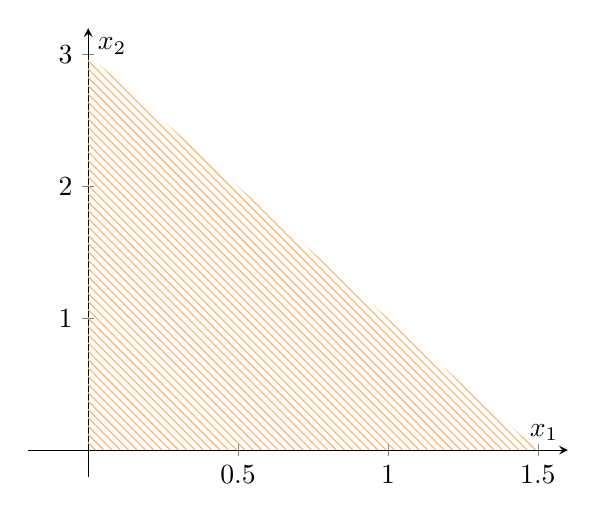
\begin{tikzpicture}
      \begin{axis}[
        axis lines=middle,
        xlabel=$x_1$,
        xmax = 1.6,
        xmin = -0.2,
        ylabel=$x_2$,
        ymax = 3.2,
        ymin = -0.2,
      ]
        \addplot[draw=none, pattern color=orange!60, pattern=north west lines] coordinates
        {(0, 0) (0, 3) (1.5, 0)};
      \end{axis}
    \end{tikzpicture}
  \end{center}
  Die Funktionen $g(x_1, x_2) \coloneqq x_1$, $h(x_1, x_2) \coloneqq x_2$,
  $j(x_1, x_2) \coloneqq 2x_1 + x_2$ sind stetig.

  Die Urbilder abgeschlossener Mengen
  \begin{flalign*}
    A_1 &= g^{-1}([0, \infty)) = [0, \infty) \times \mathbb{R} & \\
    A_2 &= h^{-1}([0, \infty)) = \mathbb{R} \times [0, \infty) \\
    A_3 &= j^{-1}((-\infty, 3]) = \qty{(x_1, x_2) \in \mathbb{R}^2 \middle|
      (x_1 \in \mathbb{R}) \land (x_2 \leq 3 - 2x_1)}
  \end{flalign*}
  sind somit abgeschlossen und
  $K = A_1 \cap A_2 \cap A_3$ ist ebenfalls abgeschlossen.
  Weiterhin ist $f$ als Komposition stetiger Funktionen ebenfalls stetig
  und es existieren Punkte $a = (a_1, a_2), b = (b_1, b_2) \in \mathbb{R}^2$
  mit $f(a) \leq f(x) \leq f(b) \forall x \in K$.

\newpage
\item $K \coloneqq \qty{x = \qty(x_1, x_2) \in \mathbb{R}^2 \middle|
    \abs{x_1 \cdot x_2} \leq 1}$ und
  $f\qty(x_1, x_2) \coloneqq \sin(x_1) + \abs{x_2}$ \\

  \textit{Lsg.}
  \begin{flalign*}
    K &= \qty{(x_1, x_2) \in \mathbb{R}^2 \middle|
         x_1 = 0 \lor x_2 \leq \frac{1}{\abs{x_1}}} & \\
      &= \qty(\bigcup_{x_1 \ne 0} \qty{x_1} \times
         \qty[-\frac{1}{\abs{x_1}}, \frac{1}{\abs{x_1}}])
         \cup \qty{\qty{0} \times \mathbb{R}}
   \end{flalign*}
   $\Rightarrow K$ ist nicht beschränkt $K$ ist nicht kompakt.

   \begin{center}
     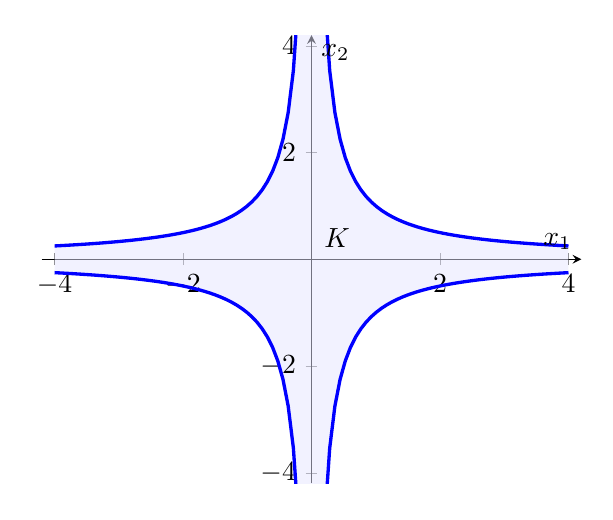
\begin{tikzpicture}[
         declare function={
           f(\x) = \x != 0 ? 1 / abs(\x) : 5;
         }
       ]
       \begin{axis}[
         axis lines=middle,
         xlabel=$x_1$,
         xmax = 4.2,
         xmin = -4.2,
         ylabel=$x_2$,
         ymax = 4.2,
         ymin = -4.2,
       ]
         \addplot[
           domain = -4:4,
           very thick,
           name path = f1,
           samples = 100,
           blue,
         ] {f(x)};
         \addplot[
           domain = -4:4,
           very thick,
           name path = f2,
           samples = 100,
           blue,
         ] { -1 *  f(x)};
         \addplot[
           fill = blue!10,
           fill opacity = .5,
         ] fill between[of = f1 and f2];
         \node at (.4,.4) {$K$};
       \end{axis}
     \end{tikzpicture}
   \end{center}

   Auch $f$ ist wegen $f(0, x_2) = \abs{x_2}, x_2 \in \mathbb{R}$
   nicht nach oben beschränkt.
   $\Rightarrow f$ besitzt kein Maximum oder Supremum auf $K$.

  \begin{minipage}[t]{.45\textwidth}
    \textbf{Fall 1}: $x_1 = 0$:
    \[
      f(x_1, x_2) = \abs{x_2} \geq 0, x_2 \in \mathbb{R}
    \]
  \end{minipage}
  \vrule
  \hfill
  \begin{minipage}[t]{.45\textwidth}
    \textbf{Fall 2}: $x_2 = 0$
    \begin{align*}
      f{x_1, x_2} &= \sin(x_1) + \abs{x_2} \geq \sin(x_1) \\
                  &= f(x_1, 0) \geq -1 \\
                  &= f\qty(2k\pi + \frac{3}{2}\pi, 0), k \in \mathbb{Z}
    \end{align*}
  \end{minipage} \\

  $f$ besitzt auf $K$ das Minimum $-1$

\end{enumerate}

\end{document}